\section{Example}
\label{subsec:example}

In this section, we show the step-by-step procedure for constructing a block-encoding using LOBE.
The example Hamiltonian is given by:
\begin{equation}
    \label{eq:example-ham}
    H = b_0^\dagger d_0(a_0^\dagger)^2 + 2 d_0^\dagger a_0^\dagger a_0 - 3 b_0^\dagger d_0^\dagger d_0
\end{equation}
with a bosonic occupancy cutoff of $\Omega = 3$.


\textbf{Step 1: Rescale Hamiltonian Coefficients for Rescaled Bosonic Ladder Operators}

First, the coefficients of the Hamiltonian are rescaled to account for the translation to the \textit{rescaled} bosonic ladder operators.
The rescaling of the coefficients is given by Eq. \ref{eq:bosonic-coeff-rescaling}.

The number of bosonic operators in each term is: $A_0 = 2$, $A_1 = 2$, and $A_2 = 0$. 
The maximum numbe of bosonic operators within a term ($A$) is $2$, occuring in the terms $T_0$ and $T_1$.
Therefore, the coefficient of the last term will be altered.

The Hamiltonian in the form of Eq. \ref{eq:bosonically-rescaled-hamiltonian} is given by:
\begin{equation}
    \tilde{H} = b_0^\dagger d_0(a_0^\dagger)^2 + 2 d_0^\dagger a_0^\dagger a_0 -  3/4 b_0^\dagger d_0^\dagger d_0
\end{equation}

The bosonic rescaling factor is given by:
\begin{equation}
    \lambda_A = (\Omega + 1)^{2/2} = 4
\end{equation}

\textbf{Step 2a: Rescale Coefficients (\textit{USP})}

In order to use \textit{USP} for the \textit{Prepare} oracle, we need to ensure that the magnitude of the coefficients are $\leq 1$.
This is done by dividing the coefficients by $\alpha^*$ (the largest coefficient magnitude).
After this process, the coefficients of the terms become: $\alpha^*_0 = 1/2$, $\alpha^*_1 = 1$, and $\alpha^*_2 = 3/4$.
The number of terms is given by $L = 3$, so the rescaling factor for this construction is $\lambda_{USP} = 4 * 2 = 8$ (Eq. \ref{eq:usp-rescaling}).

\textbf{Step 2b: Rescale Coefficients (\textit{ASP})}

If the \textit{ASP} protocol is used for the \textit{Prepare} oracle, we rescale the coefficients by dividing by the L1-norm of the coefficients (Eq. \ref{eq:asp-coeff-rescale}).
The rescaling factor for this construction is $\lambda_{ASP} = |1| + |2| + |-3/4| = 15/4$.
The rescaled coefficients then become: $\bar{\alpha}_0 = 4/15$, $\bar{\alpha}_1 = 8/15$, and $\bar{\alpha}_2 = -1/5$.

\textbf{Step 3: Construction of LOBE Select Oracle}

\begin{figure}[h]
    \label{fig:example-select}
    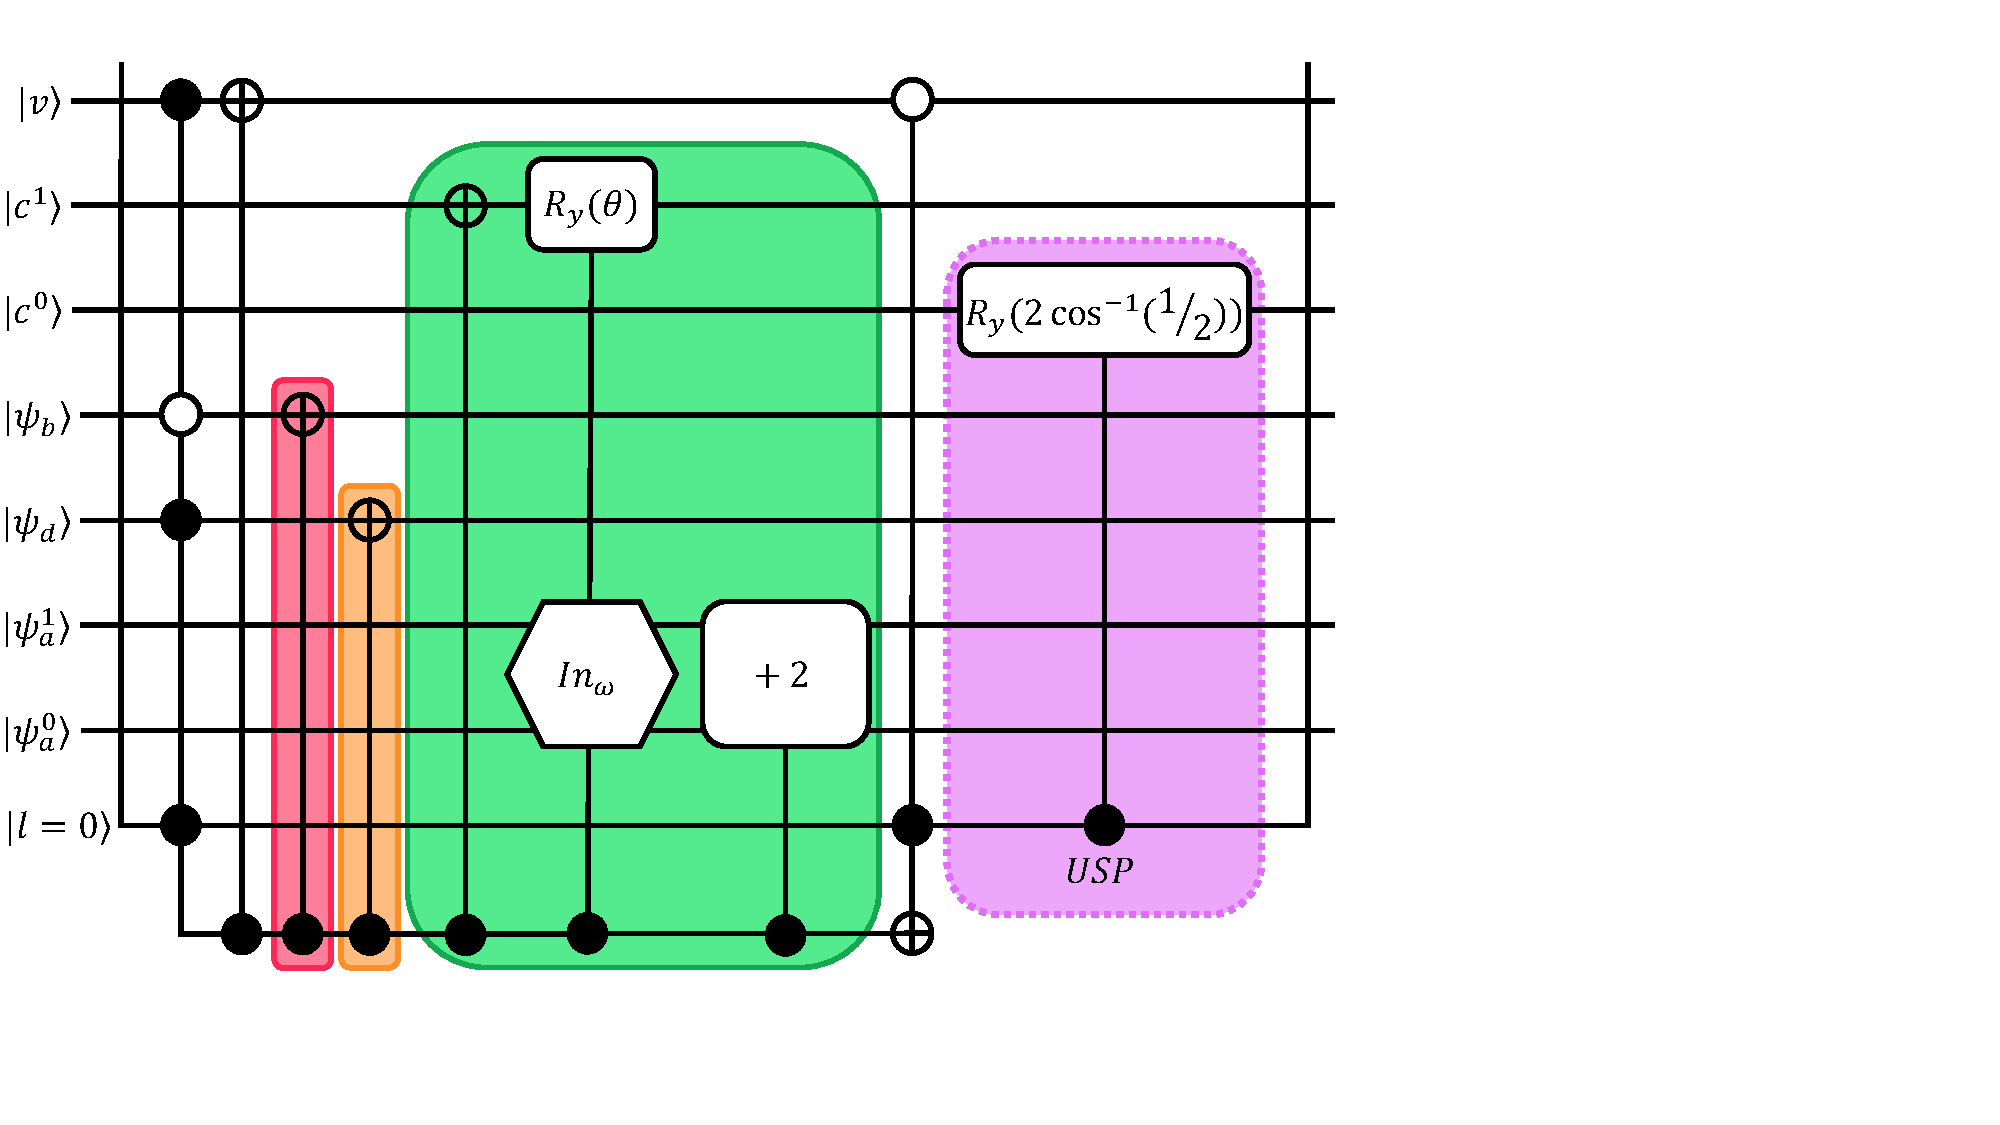
\includegraphics[height=4.5cm]{figures/T0.pdf}
    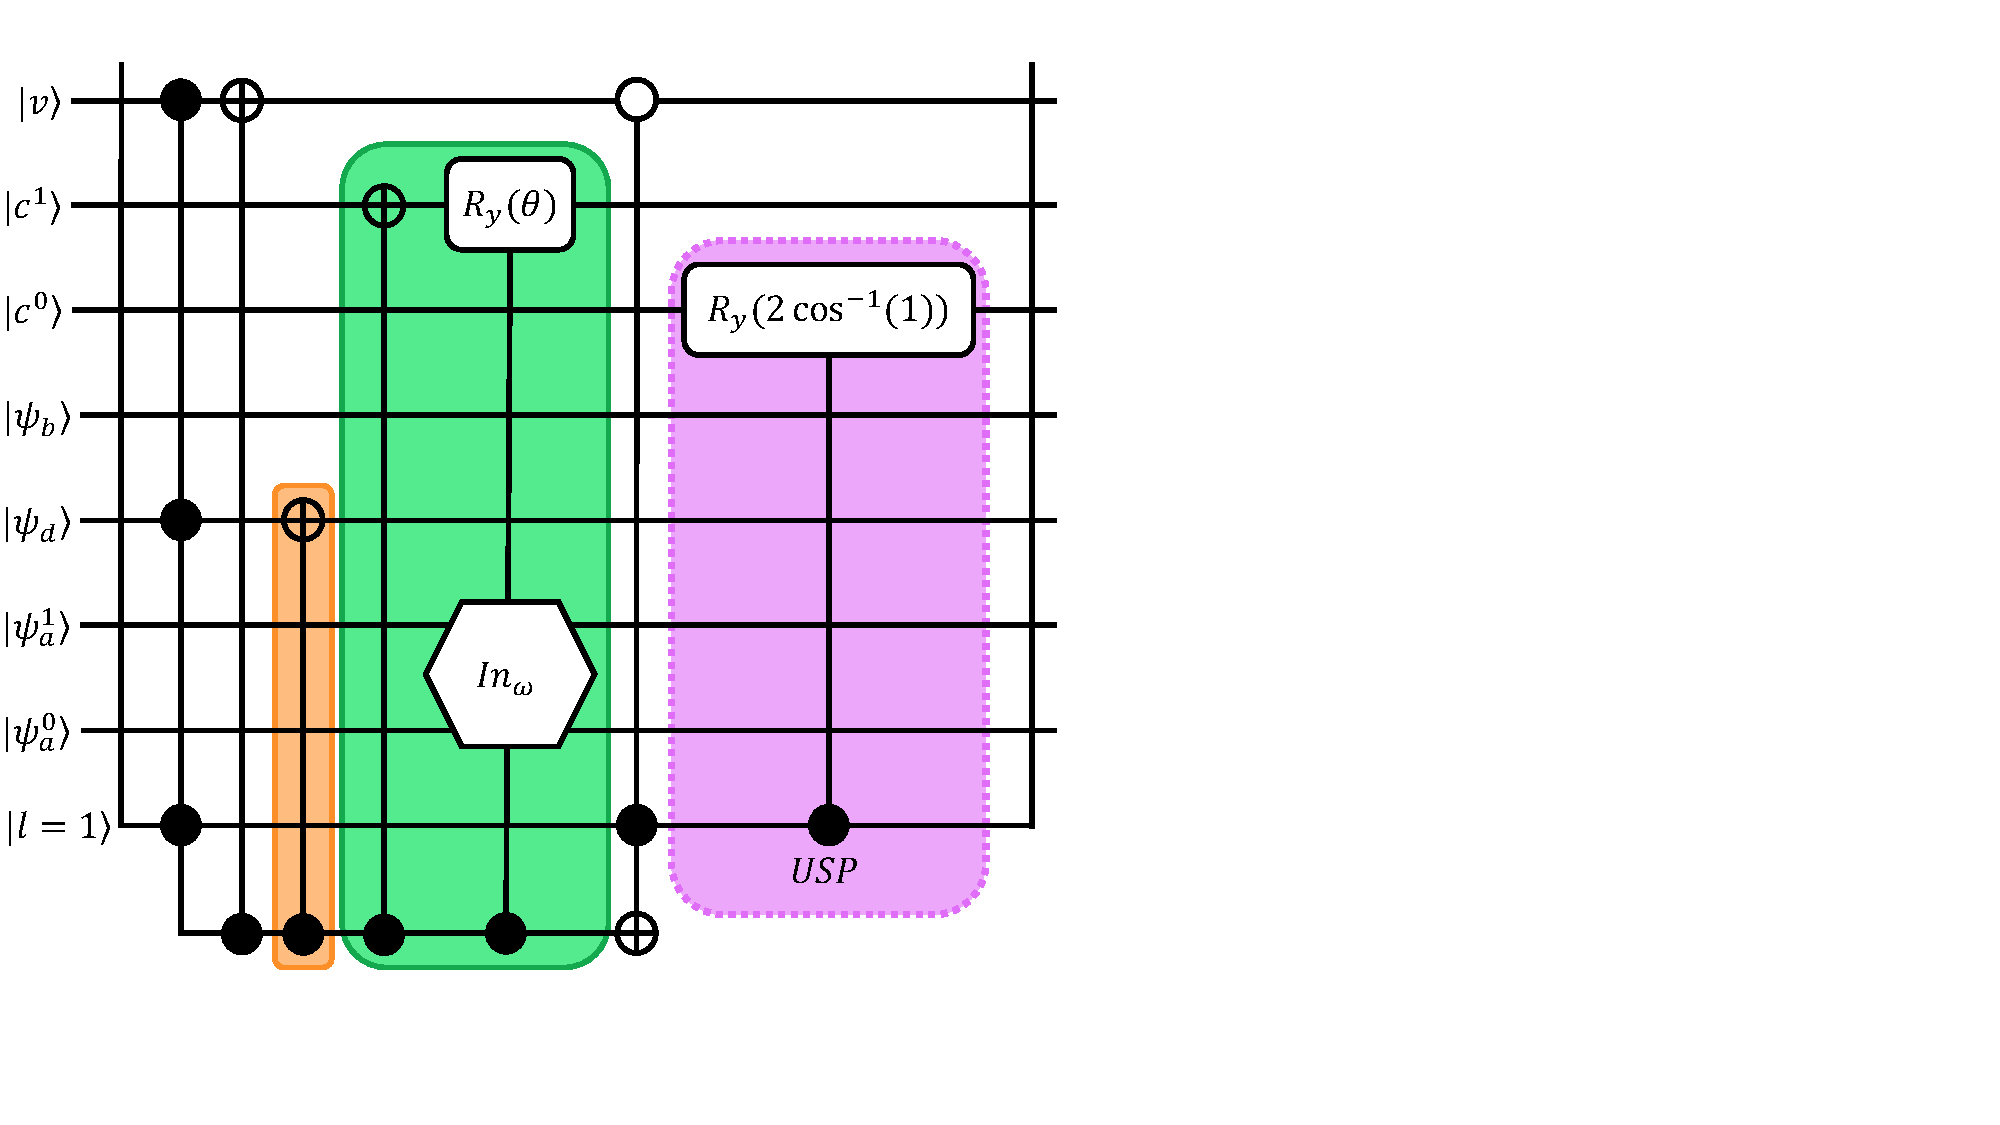
\includegraphics[height=4.5cm]{figures/T1.pdf}
    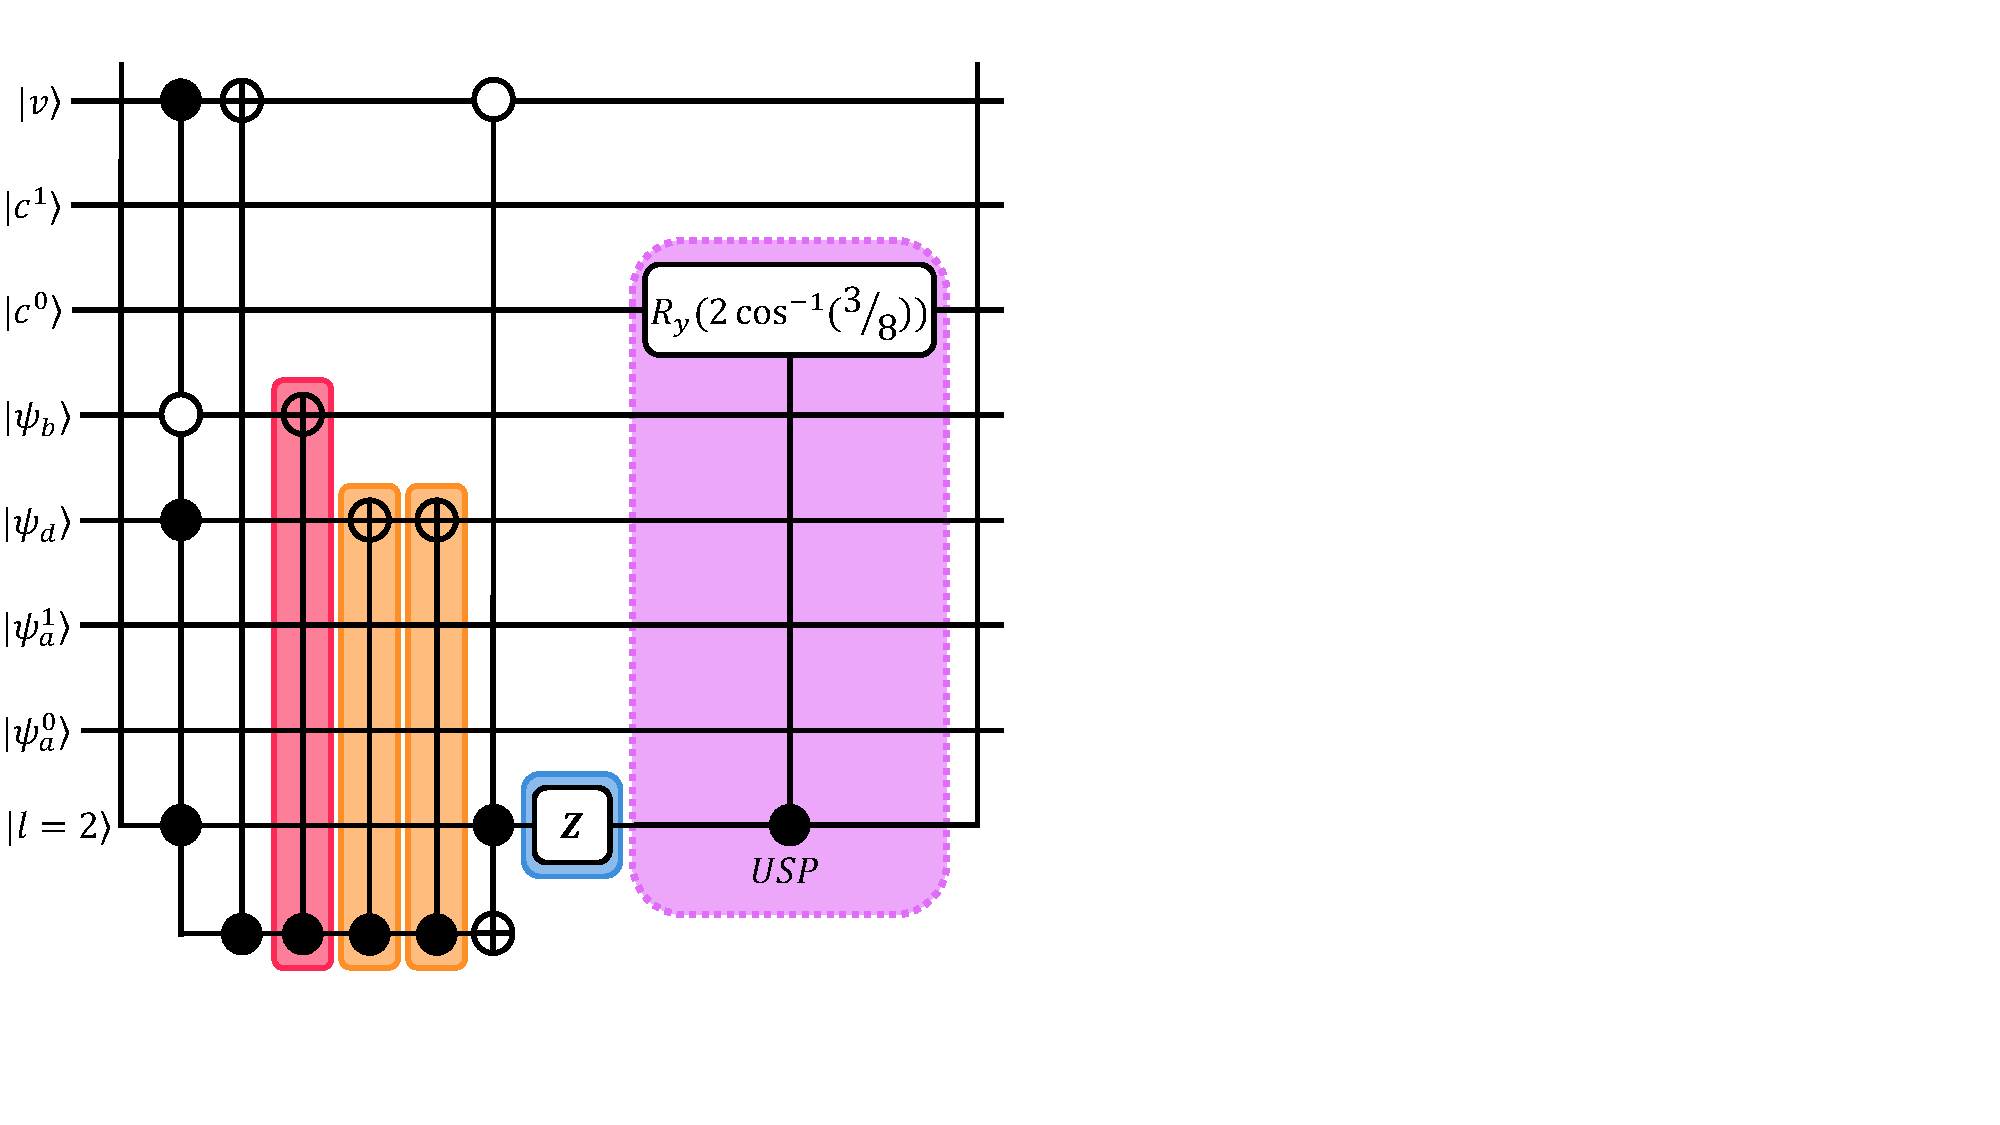
\includegraphics[height=4.5cm]{figures/T2.pdf}
    \caption{
        \textbf{Construction of Select (Example)}
        Explicit circuit constructions for the components of the \textit{Select} oracle in LOBE are shown for the example Hamiltonian.
        The circuit for apply the term $T_0 = b_0^\dagger d_0(a_0^\dagger)^2$ is shown in the left subfigure with the coefficient for the term in the \textit{USP} variant being $1/2$.
        The circuit for apply the term $T_1 = d_0^\dagger a_0^\dagger a_0$ is shown in the middle subfigure with the coefficient for the term in the \textit{USP} variant being $1$.
        The circuit for apply the term $T_2 = - b_0^\dagger d_0^\dagger d_0$ is shown in the right subfigure with the coefficient for the term in the \textit{USP} variant being $3/4$.
    }
\end{figure}

For this Hamiltonian, the three unitaries within the \textit{Select} oracle are shown in Figure \ref{fig:example-select}.
The circuit for applying the first term ($T_0$) is shown in the left subfigure. 
The circuit for applying the second term ($T_1$) is shown in the middle subfigure. 
The circuit for applying the third term ($T_2$) is shown in the right subfigure. 
The multiplexor over the index register is not shown explicitly, but generates the ancilla qubit $\ket{l == i}$ in each figure.

Using the notation in \ref{eq:gate-counts}, the preceeding three unitaries have the following gate counts:

\begin{center}
    \begin{tabular}{ |p{2cm}||p{3cm}|p{3cm}|}
        \hline
        $C$& USP &ASP\\
        \hline
        $U_{T_0}$   & $(8, 8, 7)$    &$(6, 8, 7)$\\
        $U_{T_0}$   & $(8, 7, 6)$    &$(6, 7, 6)$\\
        $U_{T_0}$   & $(2, 4, 3)$    &$(0, 4, 3)$\\
        \hline
        $C_{\text{SELECT}}$ & $(18, 21, 18)$ &$(12, 21, 18)$\\
        $C_{\text{PREPARE}}$ & $(0, 0, 0)$ &$(3, 0, 0)$\\
        \hline
        $C_{\text{Total}}$ & $(18, 21, 18)$& $(18, 21, 18)$\\
        \hline
       \end{tabular}
\end{center}

Note that the counts for $C_{\text{SELECT}}$ are not simply the sum of the cost of the unitaries above because we must add the cost of the controlled multiplexor over the index register.
For this example, the cost of the controlled-multiplexor is two more left and right elbows ($N_{elbows} = L$). 

\textbf{Step 5: Post-Processing}

As a result of the various rescaling factors, the encoded matrix within the block-encoded is a rescaled matrix based on Eq. \ref{eq:post-process}.
In the case of \textit{USP}, the full rescaling factor is given by: $(\lambda_A * \lambda_{USP}) = 4*8 = 32$.
In the case of \textit{ASP}, the full rescaling factor is given by: $(\lambda_A * \lambda_{ASP}) = 4*15/4 = 15$.
In the context of computing the eigenvalues of the Hamiltonian given the eigenvalues of the rescaled Hamiltonian, we can post-process the rescaled eigenvalues by $E = 32 \bar{E}_{USP} = 15 \bar{E}_{ASP}$.